\chapter{Estado del arte}

\section{Test de Guralnik o SPPB}

\subsection{¿Qué es SPPB?}
El doctor Guralnik JM, junto a otros compañeros, desarrolló un test al que denominó ``Short physical performance battery'' y que consiste en un conjunto de pruebas físicas con el objetivo de evaluar el equilibrio, fuerza, marcha y resistencia en el paciente\cite{SPPB_nlm}. Las pruebas serían las siguientes:

\begin{enumerate}
  \item \textbf{Equilibrio:} Se divide a su vez en tres partes según la posición de los pies, que puede ser juntos, semi-tándem y tándem. Mide la habilidad para mantenerse erguido en cada una durante diez segundos. 
  \item \textbf{Velocidad de marcha:} Mide el tiempo invertido en caminar tres o cuatro metros. Hay que realizarla dos veces y quedarse con el mejor resultado (menor tiempo).
  \item \textbf{Levantarse y sentarse en una silla:} Mide el tiempo invertido en levantarse y volver a sentarse cinco veces en una silla.
\end{enumerate}

En cada una de las pruebas se puede obtener una puntuación que varía desde los cero hasta los cuatro puntos, siendo doce la cantidad total que se puede conseguir en el mejor de los casos. Además, muchos estudios dividen el resultado en cuatro clasificaciones de limitación física, que pueden ser desde grave (0-3 puntos), moderada (4-6 puntos), leve (7-9 puntos) y mínima (10-12 puntos)\cite[Pag 8]{SPPB_clasificacion}. Una puntuación que se encuentre por debajo de 10 es indicativo de fragilidad. Además, aunque se produzcan cambios que involucren un único punto, es importante tenerlos en cuenta porque podrían tener significado clínico\cite{juntandalucia}.

Para el estudio, se solicitó la participación de un grupo formado por 5000 adultos con una edad de 71 años o superior, a los que se le pidió realizar el test. Los resultados arrojaron una clara relación entre los auto-informes de discapacidad y la puntuación obtenida, sirviendo a la misma vez como predictores independientes de mortalidad. \cite{SPPB_nlm}

\subsection{Uso y aceptación del test SPPB}

En la actualidad, el test SPPB es un indicador de fragilidad sobradamente aceptado y su uso está muy extendido. En España, el Ministerio de Sanidad, Servicios Sociales e Igualdad presentó en 2014 el \textit{Documento de consenso sobre prevención de fragilidad y caídas en la persona mayor: estrategia de promoción de la salud y prevención en el Sistema Nacional de Salud (SNS)}, implantado de forma imperativa en los Sistemas de Salud autonómicos\cite[Pag 27-28]{Fragilidad_y_nutricion}, en el que se insta a utilizar de forma preferente el test \textbf{Short Physical Performance Battery} para realizar un cribado inicial de la fragilidad o limitación funcional en ancianos\cite[Pag 21]{ministerio_sanidad}.

Es por tanto una de las principales técnicas para determinar si el paciente sufre algún tipo de fragilidad precoz cuando acude a consultas de atención primaria debido, entre otras cosas, a su comprobada eficacia, a no requerir de material especializado y a la rapidez de ejecución, sobre todo útil en clínicas que se encuentran saturadas\cite{predictive_sppb}. 

No obstante, y a pesar de ser un test fácil de realizar, no es común que los ancianos lo lleven a cabo de forma autónoma en sus hogares. De hacerse, podría ser realmente útil para que ellos mismos mantengan un seguimiento de su estado físico y tomen las medidas oportunas ante un deterioro, como visitar al médico y realizar más ejercicio. Por supuesto, con esto no se buscaría reemplazar el diagnóstico de un experto, sino precisamente encontrar el problema a tiempo para acudir cuanto antes a un centro especializado.

Posiblemente, algunas de las razones para no encargar hasta ahora la ejecución del test de forma independiente a los ancianos sean: la necesidad de explicar y ejecutar de forma correcta las pruebas, el uso de un cronómetro para medir el tiempo y aplicar correctamente el sistema de puntos.

\newpage
\section{Android}
\subsection{¿Qué es Android?}

``Android es un sistema operativo móvil desarrollado por Google, basado en el Kernel de Linux y otros software de código abierto. Fue diseñado para dispositivos móviles con pantalla táctil, como teléfonos inteligentes, tabletas, relojes inteligentes, automóviles y televisores.

Inicialmente fue desarrollado por Android Inc., empresa que Google respaldó económicamente y que adquirió en 2005. Android fue presentado en 2007 junto con la fundación del Open Handset Alliance (un consorcio de compañías de hardware, software y telecomunicaciones) para avanzar en los estándares abiertos de los dispositivos móviles. La versión básica de Android es conocida como Android Open Source Project (AOSP). Android es el sistema operativo móvil más utilizado del mundo, con una cuota de mercado superior al 80\% al año 2017, muy por encima de iOS.''
\begin{flushright}
    (Wikipedia, 13 de Agosto de 2019. \cite{android_wikipedia})
\end{flushright}

\subsection{Arquitectura}
El sistema operativo Android tiene una arquitectura basada en Linux como acabamos de ver. Está formado por estos seis componentes principales, que pueden consultarse en la figura \ref{fig:arquitectura}\cite{arquitecturaAndroid}:

\begin{itemize}

    \item \textbf{Kernel de linux:} Es la base del sistema operativo. Android, al estar basado en un kernel ya conocido, facilita el trabajo de los desarrolladores de hardware. Otras muchas partes, como el \textit{tiempo de ejecución de Android}, utilizan esta base para llevar a cabo funcionalidades que pueden ir desde la generación de subprocesos hasta la administración de memoria de bajo nivel. 
    
    \item \textbf{Capa de abstracción de hardware (HAL):} Como su propio nombre nos sugiere, la capa de abstracción de hardware se encarga de presentar una interfaz que facilita el uso y expone las capacidades hardware de cada dispositivo al framework de la Java API. Está conformada por distintos módulos de biblioteca (figura 3.1, Hardware Abstraction Layer), cada uno de ellos destinados a implementar la interfaz para un elemento concreto del hardware, como puede ser el audio, el bluetooth o los sensores (entre ellos el acelerómetro, el cual usará nuestra aplicación).
    
    \newpage
    
    \item \textbf{Tiempo de ejecución de android:} A partir de la API 21 de Android, se produjo un cambio que provocó que desde ese momento, ``cada aplicación ejecutase sus propios procesos con sus propias instancias del tiempo de ejecución de android (ART)''\cite{arquitecturaAndroid}. ART podía ejecutar múltiples máquinas virtuales con archivos llamados DEX, un tipo nuevo de formato cuyo objetivo es ocupar el mínimo espacio posible, dando la posibilidad de que esto ocurriese incluso en teléfonos con poca memoria. Algunas de las opciones que ofrece ART son un recolector de elementos no usados (GC), compilación AOT y JIT (Ahead-of-time y Just-in-time), y una mayor compatibilidad de depuración.
    
    \item \textbf{Bibliotecasm nativas de C y C++:} En android, múltiples componentes centrales como pueden ser la capa de abstracción de hardware (HAL) o el tiempo de ejecución de android (ART) requieren de bibliotecas nativas que están escritas en C y C++. Por ello, Android da la posibilidad de ofrecer la funcionalidad de estas bibliotecas nativas a las apps mediante la API del framework de Java.
    
    \item \textbf{Framework de la Java API:} Android ofrece una serie de APIs de Java con las que se pueden llevas a cabo prácticamente todos los aspectos de la creación de una aplicación. Además, permiten simplificar la reutilización de los siguientes módulos y servicios que ofrece el sistema operativo, \textbf{algunos} de los cuales son:
    \begin{itemize}
        \item \textbf{Un conjunto de vistas} con el que diseñar e implementar la interfaz de usuario de la aplicación. Posee muchos elementos como pueden ser cuadros de texto, barras de progresión, imágenes y botones. Su uso es muy sencillo.
        \item \textbf{Un administrador de recursos} para acceder a elementos que no poseen código. De esta forma, se pueden encontrar los strings, las imágenes, archivos XML, etc. Esto permite agrupar en un mismo lugar todos los recursos de cada tipo, de modo que si al cambiar uno de ellos, todas las partes de la aplicación que hagan uso de él se actualizarán con la nueva información, facilitando la administración del mismo al no tener que ir buscándolo archivo por archivo.
        \item \textbf{Administrador de notificaciones}, que facilita la programación personalizada de información que pueda ser mostrada en la barra de estado.
    \end{itemize}
    
    \item \textbf{Aplicaciones del sistema:} Se trata del conjunto de aplicaciones que hay instaladas en el sistema, independientemente de si lo están de forma nativa o de si es el propio usuario quien las descarga e instala. 
\end{itemize}


\begin{figure}[H]
	\centering
	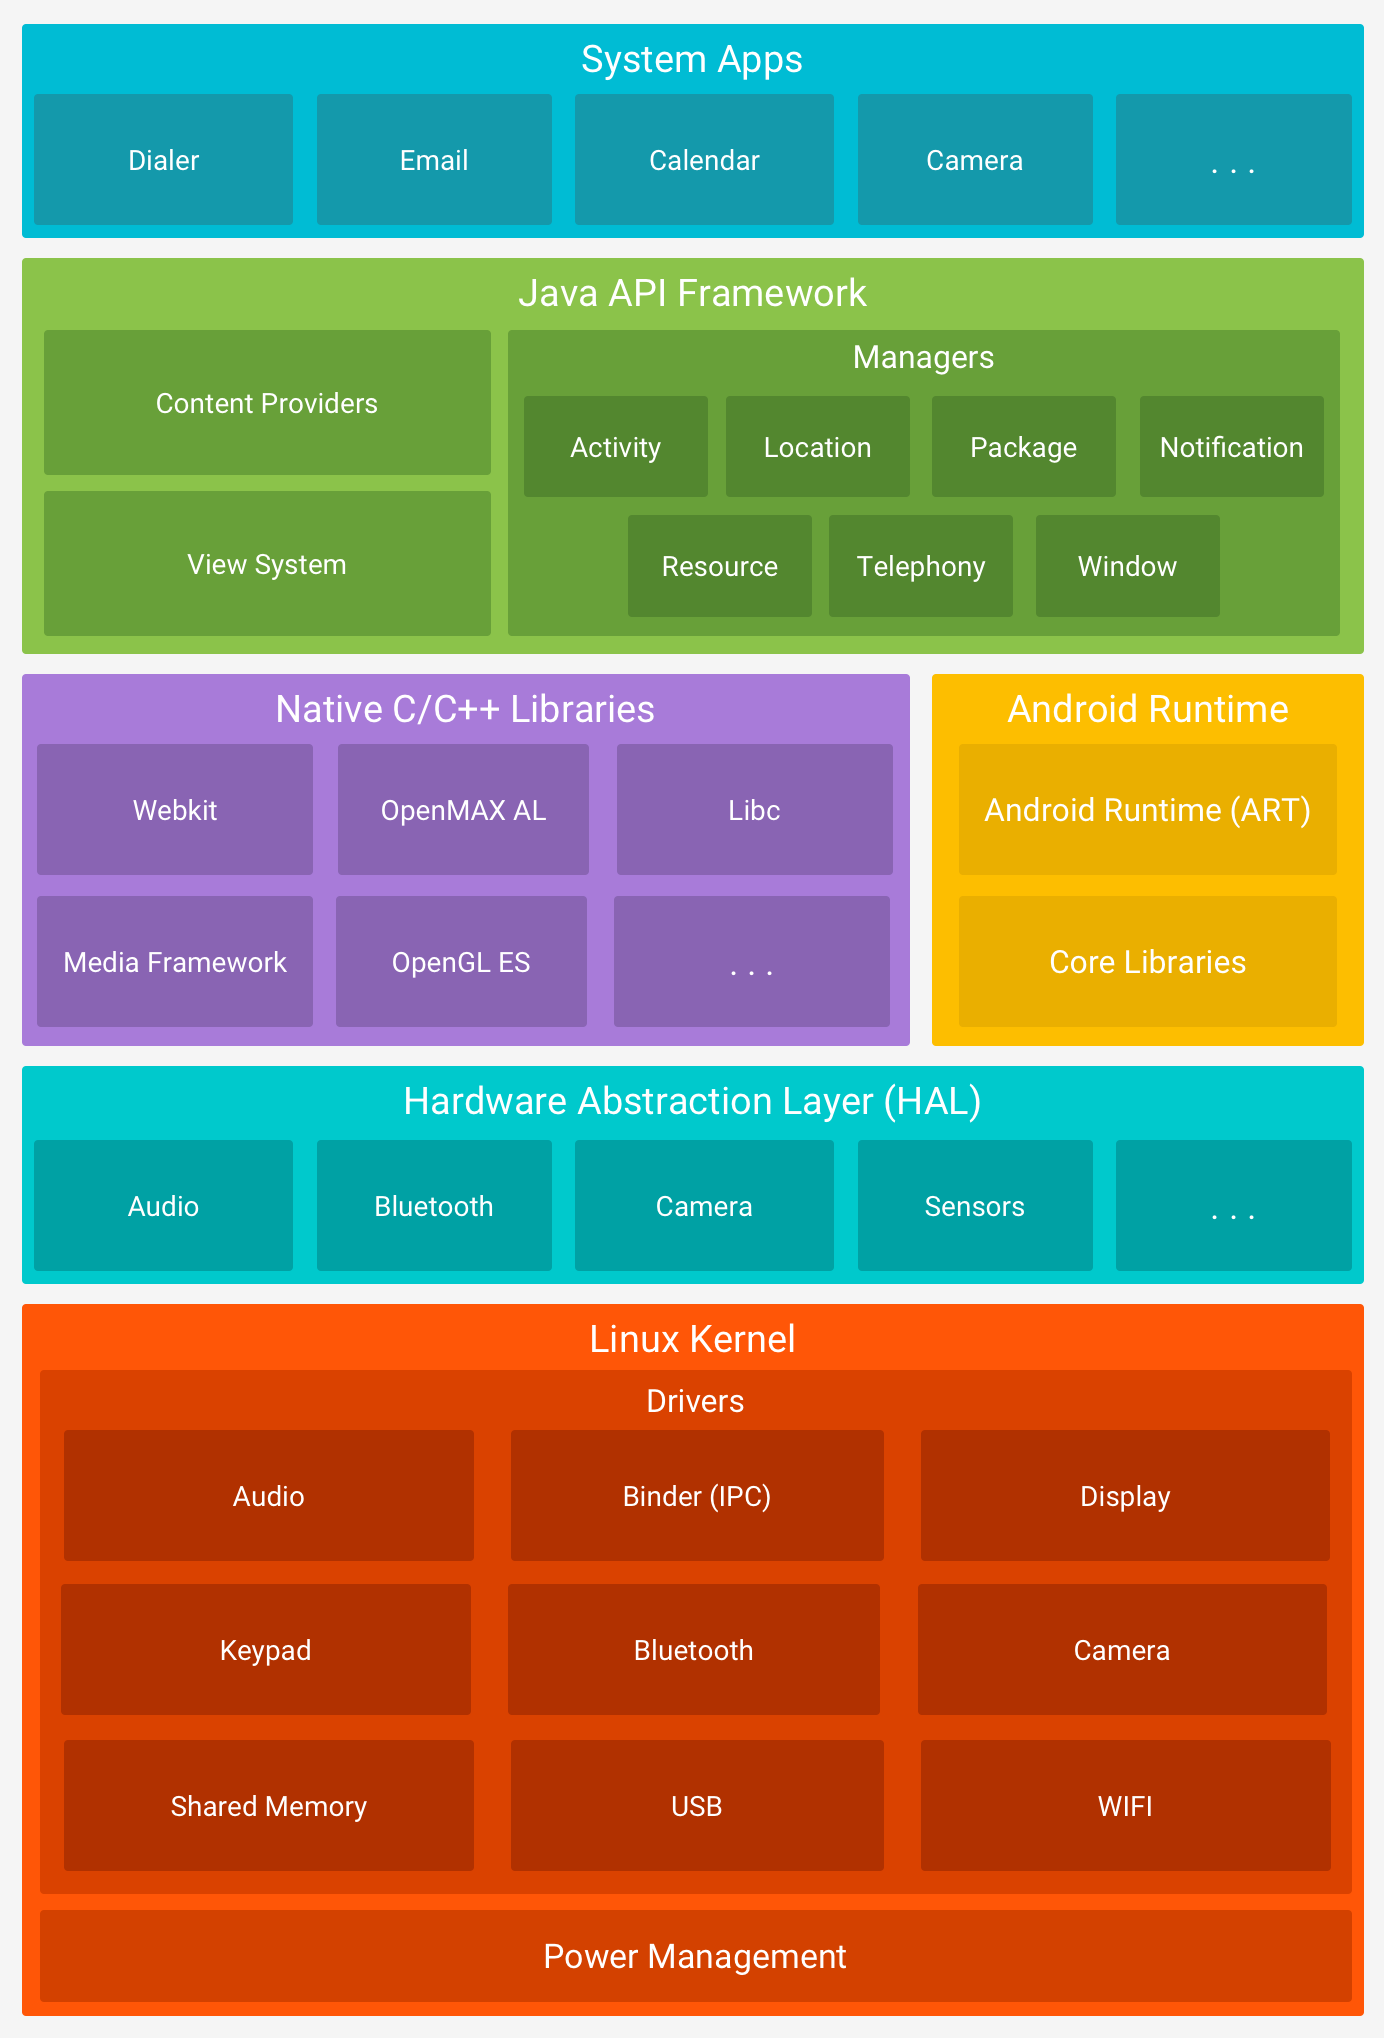
\includegraphics[scale=0.25]{imagenes/android-stack_2x.png}
	\caption{Pila de software de Android\cite{arquitecturaAndroid}\label{fig:arquitectura}}
\end{figure}

\subsection{Distribución de Android}
La distribución de Android viene a mostrarnos cual es el número de dispositivos que usan cada una de las versiones de Android. De hecho, el gran problema que aún presenta este sistema operativo es que pocos son los sistemas actualizados a la última versión disponible si los comparamos con el total, resaltando aún más al fijarnos en las estadísticas de iOS, el sistema de Apple, cuyos usuarios adoptan rápidamente la versión más reciente al poco tiempo de ser publicada. 

Gran parte de la culpa reside en el amplísimo número de marcas privadas que fabrican teléfonos con Android, cada una de las cuales con su propio hardware y su idea de cómo y cuando debería actualizar sus dispositivos. Esto acaba produciendo que muchas marcas sólo se preocupen de sus móviles más caros, y durante poco tiempo, creando un gran banco de usuarios con versiones de software desactualizadas, fallos de seguridad y sin las últimas novedades. 

Las estadísticas de distribución más recientes hasta el momento fueron publicadas en mayo de 2019, y son las siguientes:
\begin{figure}[H]
	\centering
	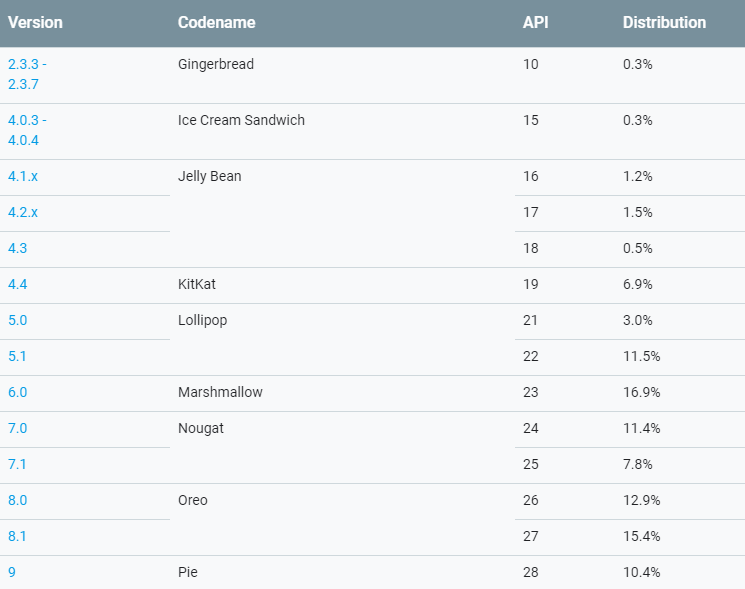
\includegraphics[scale=0.65]{imagenes/distribucion.png}
	\caption{Distribución de las versiones Android\cite{dashboards}\label{fig:distribucion}}
\end{figure}


\section{Opciones actuales en el mercado}

Son múltiples las guías y manuales sobre el test SPPB que se pueden encontrar en internet, donde se explica de forma detallada cuales son los pasos a tomar en cada prueba, los tiempos y los puntos. 

Sin embargo, no pasa igual si buscamos entre las aplicaciones de Google Play el término "SPPB". A pesar de ser el sistema operativo más usado del mundo, sólo dos de los resultados de la búsqueda están de algún modo relacionados con la valoración de fragilidad en ancianos, como se puede observar en la figura \ref{fig:google_play}. De ellas, no comentaremos la aplicación denominada ``Valoración de la Fragilidad''\cite{BlueBliss} puesto que en la práctica no posee ninguna opción para realizar el test SPPB.

\begin{figure}[H]
	\centering
	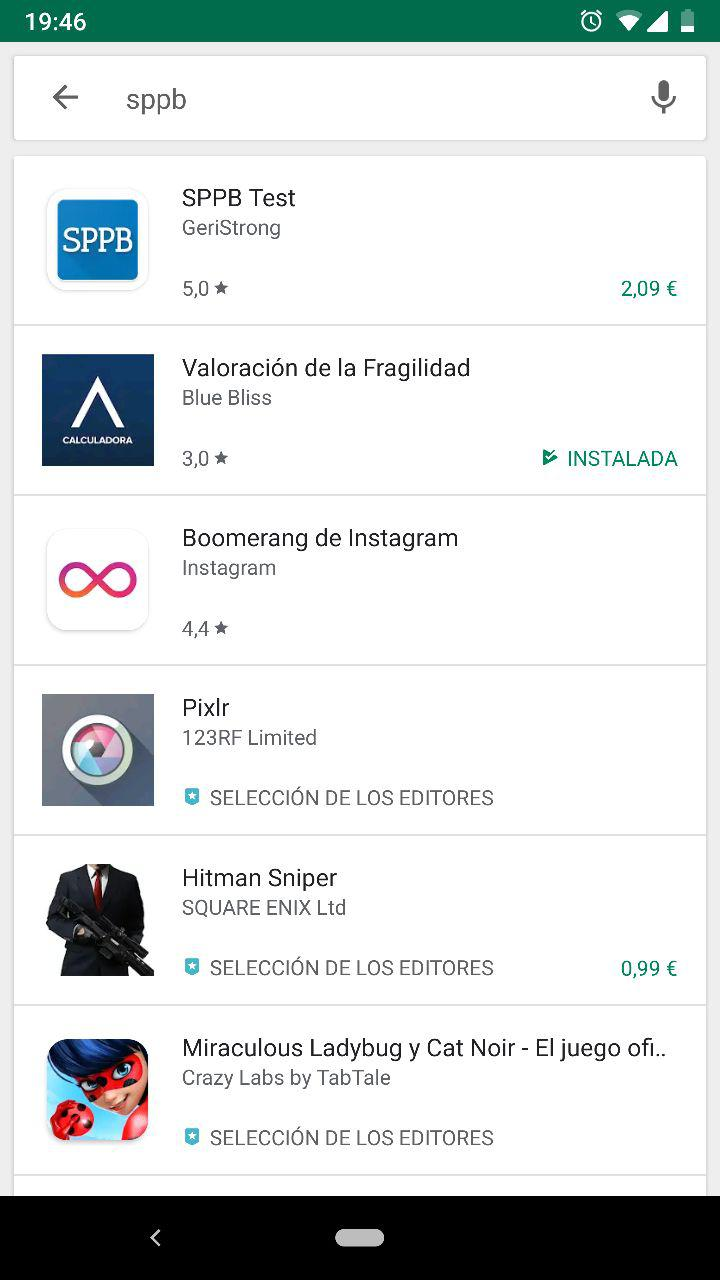
\includegraphics[scale=0.35]{imagenes/googlePlay_resultado.jpg}
	\caption{Resultados al buscar SPPB en la Google Play\label{fig:google_play}}
\end{figure}

La primera aplicación, de nombre ``SPPB Test''\cite{GeriStrong}, está enteramente dedicada a la realización y ejecución del test de Guralnik. Sin embargo, una primera pega que encontramos es su no gratuidad, que podría convertirse en un impedimento si pretendiésemos su uso entre la población anciana. A esto hay que sumarle que no es un proyecto de código abierto, con lo que no cabe la posibilidad de presentar mejoras ajenas a las que introduzca el propio creador.

\begin{figure}[H]
	\centering
	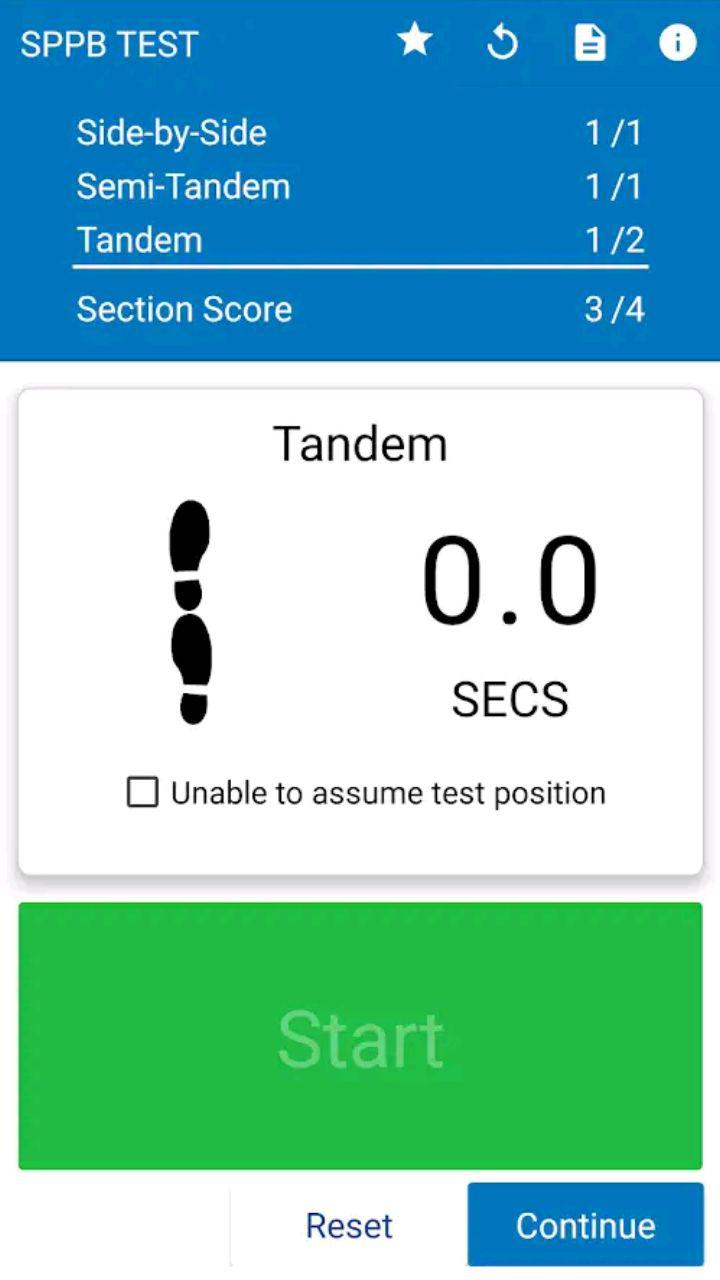
\includegraphics[scale=0.35]{imagenes/sppb_geristrong.jpg}
	\caption{Aplicación SPPB Test de GeriStrong\cite{GeriStrong}\label{fig:geriStrong}}
\end{figure}

Por otra parte, la aplicación parece sencilla de usar y ahorra la necesidad de elementos como un cronómetro o calculadora. Su enfoque está dirigido hacia el uso por parte de un médico o profesional, que guíe al paciente a través de las diferentes pruebas y controle la aplicación en todo momento. Además, es esa persona la encargada de comprobar y validar los movimientos que realiza el paciente, determinando si no se han llevado a cabo correctamente.

\section{Propuesta}

La propuesta que nosotros presentamos es la de crear una aplicación abierta y de código libre, sin ningún coste de compra, que esté orientada tanto al uso autónomo por parte de los ancianos como a su uso vigilado por un profesional. Además será muy importante la \textbf{integración del acelerómetro} presente en los móviles, que deberá encargarse de comprobar y validar la ejecución correcta de cada prueba.

Para conseguirlo, algunos de los puntos más importantes serán:
\begin{enumerate}
  \item Explicación clara y concisa del funcionamiento de cada una de las pruebas, tanto de forma escrita como mediante instrucciones guiadas por voz.
  \item Uso del acelerómetro para comprobar si cada prueba se ejecuta de forma correcta.
  \item Diseño bonito y adaptado a las pautas ofrecidas por Android.
  \item Posibilidad de guardar los resultados de múltiples usuarios.
\end{enumerate}